\section{Quantum chromodynamics (QCD)}
The Quantum Chromodynamics (QCD) is the fundamental theory of the strong interaction.
It describes the interaction of objects that carries color charges. 
Quarks and gluons are the fundamental degrees of freedom of the theory. 
Quarks are fermions and gluons are bosons that mediate the interaction between color charges.
The QCD Lagrangian (with one flavor of quark) is,
\begin{eqnarray}
\mathcal{L} = \bar{\psi_i} \left(i\gamma_\mu D^\mu_{ij} -m \delta_{ij} \right)\psi_j - \frac{1}{4}G_{\mu\nu}^a G^{\mu\nu,a},
\end{eqnarray}
where $\psi_i$ the Dirac spinor of the quark field with color $i = 1,2,\cdot N_c$. 
\begin{eqnarray}
D^\mu = \partial^\mu - i g T^a A^{\mu, a}
\end{eqnarray}
is the covariant derivative which contains the interaction between quark field and the gluon field.
The pure gauge term involving the field tensor,
\begin{eqnarray}
G^{\mu\nu,a} = \partial^\mu A^{\nu, a} - \partial^\nu A^{\mu, a} + g f^{abc} A^{\mu,b}A^{\mu,c}
\end{eqnarray}
contains the kinematic term and the self interaction of the gluon field.
The non-linearity of the gluon self interaction comes from its non-abliaen nature, manifesting as the structure constant $f^{abc}$.
The Feynman rule for QCD is summarized as follows,
\begin{figure}
    \centering
    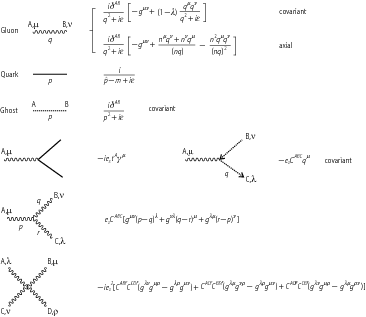
\includegraphics{qcd-feynman-rules.png}
    \caption{Caption}
    \label{fig:qcd-feynman}
\end{figure}

Due to quantum fluctuations, the coupling constant of the quantum field theory runs with the resolution, i.e., energy scale. 
In perturbation theory, the running of the strong coupling constant, characterized by the $\beta$-function, can be calculated order by order, 
\begin{eqnarray}
\frac{\partial g}{\partial \ln\mu} = \beta(g).
\end{eqnarray}
At leading order, the QCD $\beta$ function with number of colors $N_c$ and $n_f$ flavors of fermions is,
\begin{eqnarray}
\beta(g) = - \left( \frac{11}{3}N_c - \frac{2}{3}n_f \right) \frac{g^3}{16\pi^2}.
\end{eqnarray}
This $\beta$ function is negative for $N_c=3$ and realistic $n_f = 2\cdots 6$, meaning the effective coupling constant decreases with increasing energy resolution.
This feature is known as the asymptotic freedom of QCD that its interaction becomes small at asymptotically high energy.
It is the asymptotic freedom that made possible the usage of perturbation theory at high energy.
Solving which yields the leading order running coupling constant $\alpha_s = g^2/4\pi$ as a function of energy scale,
\begin{eqnarray}
    \alpha_s(\mu^2) = \frac{4\pi}{\left(\frac{11}{3}N_c - \frac{2}{3}n_f\right)\ln\left(\frac{Q^2}{\Lambda^2}\right)}
\end{eqnarray}
With the integration constant absorbed into the QCD energy scale $\Lambda$, determined by experimental measurements. 
At leading order $\Lambda \approx 200$ MeV.
Before hitting this energy scale, the coupling constant is already becoming too large for reliable perturbative calculations.
$\Lambda$ is often an estimation of the non-perturbative scale of QCD.

\begin{figure}
    \centering
    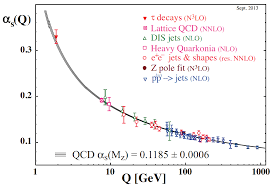
\includegraphics{alphas.png}
    \caption{Caption}
    \label{fig:alphas}
\end{figure}

At low energy $Q\sim \Lambda$ or large distance, the theory enters the non-perturbative regime. 
The coupling between color charges is so large that isolated color cannot exist alone without its strong color field constantly populating more color objects.
The color charges combined to form colorless QCD bound states known as hadrons, such as protons, neutrons and pions.
Depending on its content valance quarks (quarks that carry the net quantum number), hadrons are generally categorized as baryons and mesons.
Baryons are hadrons with three valance quarks or anti-quarks, while mesons consist of a valance quark and an anti-quark.
Besides valance quarks, hadrons are also populated with sea quarks pairs and gluons due to quantum fluctuations.
The physics of non-perturbative regime cannot be obtained from perturbative QCD and the only reliable way nowadays is lattice QCD technique where the QCD Lagrangian is discretized on a finite lattice and studied on a computer.

\section{The QCD phase diagram}
Ever since QCD is proposed to be the fundamental theory of strong interaction (and therefore nuclear physics) and the discover of asymptotic freedom, people have been questing for the phase structure of nuclear matter. 
The phase-diagram is often studied with temperature and baryon chemical potential as independent variables. 
The phase structure on the landscape of independent thermodynamic quantities such as isospin asymmetry, strangeness, etc have also attract great attentions.
Ordinary nuclear matter (nuclei) are many body bound states at zero temperature and Baryon chemical potential $\mu_B\approx 1$ GeV.
A first insight at finite temperature is that because the weakening of the coupling at high energy scale, the nuclear matter was thought to transit from hadronic matter to a system of liberated quarks and gluons, termed the quark-gluon plasma (QGP). 
Lattice QCD calculations have studied this transition at zero baryon chemical potential with physical parameters.
Figure \ref{fig:qcd_eos} quotes the results obtained from the HotQCD Collaboration.
It shows the pressure, energy density and entropy density of the 2+1 flavor QCD.
The thermodynamic quantities scaled by powers of temperature can be understood as the effect number of degrees of freedom.
The non-interacting limit (ideal gas of quarks and gluons) is denoted as the dashed lines. 
It is observed that the lattice results converges to the expectation from a hadron resonance gas model (HRG) at low temperature and smoothly transit to higher values in a narrow temperature range around the pseudo critical temperature $T_c \approx 150 $ MeV, suggesting an increase of degrees of freedom.

This transition is a cross-over type phase transition at vanishing baryon chemical potential.
At finite baryon chemical potential, the lattice QCD is faced with the fermion sign problem. But many phenomenological models and Dyson-Schwinger equations studies have suggested the existence of a first order phase transition at large $\mu_B/T$.
If such a first order phase transition exist, the coexistence line must end at some point when decreasing $\mu_B/T$, approaching the cross-over phase transition established from lattice study.
Such a point, called the critical end point (CEP), is of great interest both theoretically and experimentally.
At high enough chemical potential (density) and low temperature, another phase of nuclear matter known as the "Color Superconductor" has been proposed, where the quarks forms Cooper pairs as those found among electrons in common superconductors.

Experimentally, colliding heavy nuclei at ultra-relativistic high energies allows one to explore the high temperature region of the phase diagram.
Since 2005, the Relativistic Heavy-ion Collider (RHIC) at the Brookheaven National Laboratory (BNL) started colliding gold nuclei at 200 GeV. 
The Large Hadron Collider (LHC) started its heavy ion programs later, colliding lead nuclei at 2.76 TeV and 5.02 TeV.
A striking discovery is that, contrary to previous expectation of weakly coupled gas of quarks and gluons, there are many evidences point that the state of matter created resembles a nearly perfect fluid in the estimated temperature range of a few times of $T_c$.
This discovery reveals the strongly coupled nature of the matter produced in relativistic nuclear collisions and has been entitled the name strongly coupled quark-gluon plasma (sQGP).
The phenomenology of relativistic heavy-ion collisions is discussed in detail in the next chapter.

\begin{figure}
    \centering
    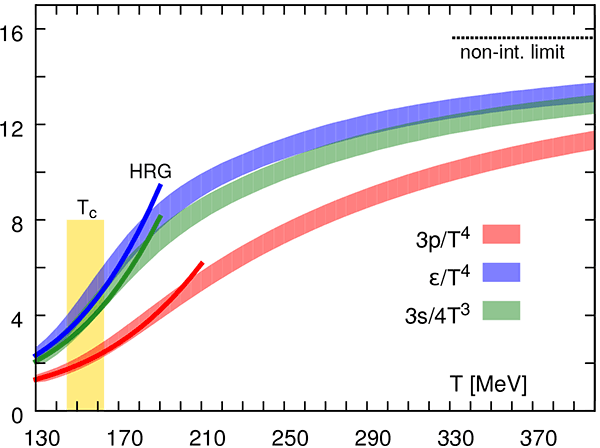
\includegraphics[width=.8\textwidth]{qcd-eos.png}
    \caption{Caption}
    \label{fig:qcd_eos}
\end{figure}

\begin{figure}
    \centering
    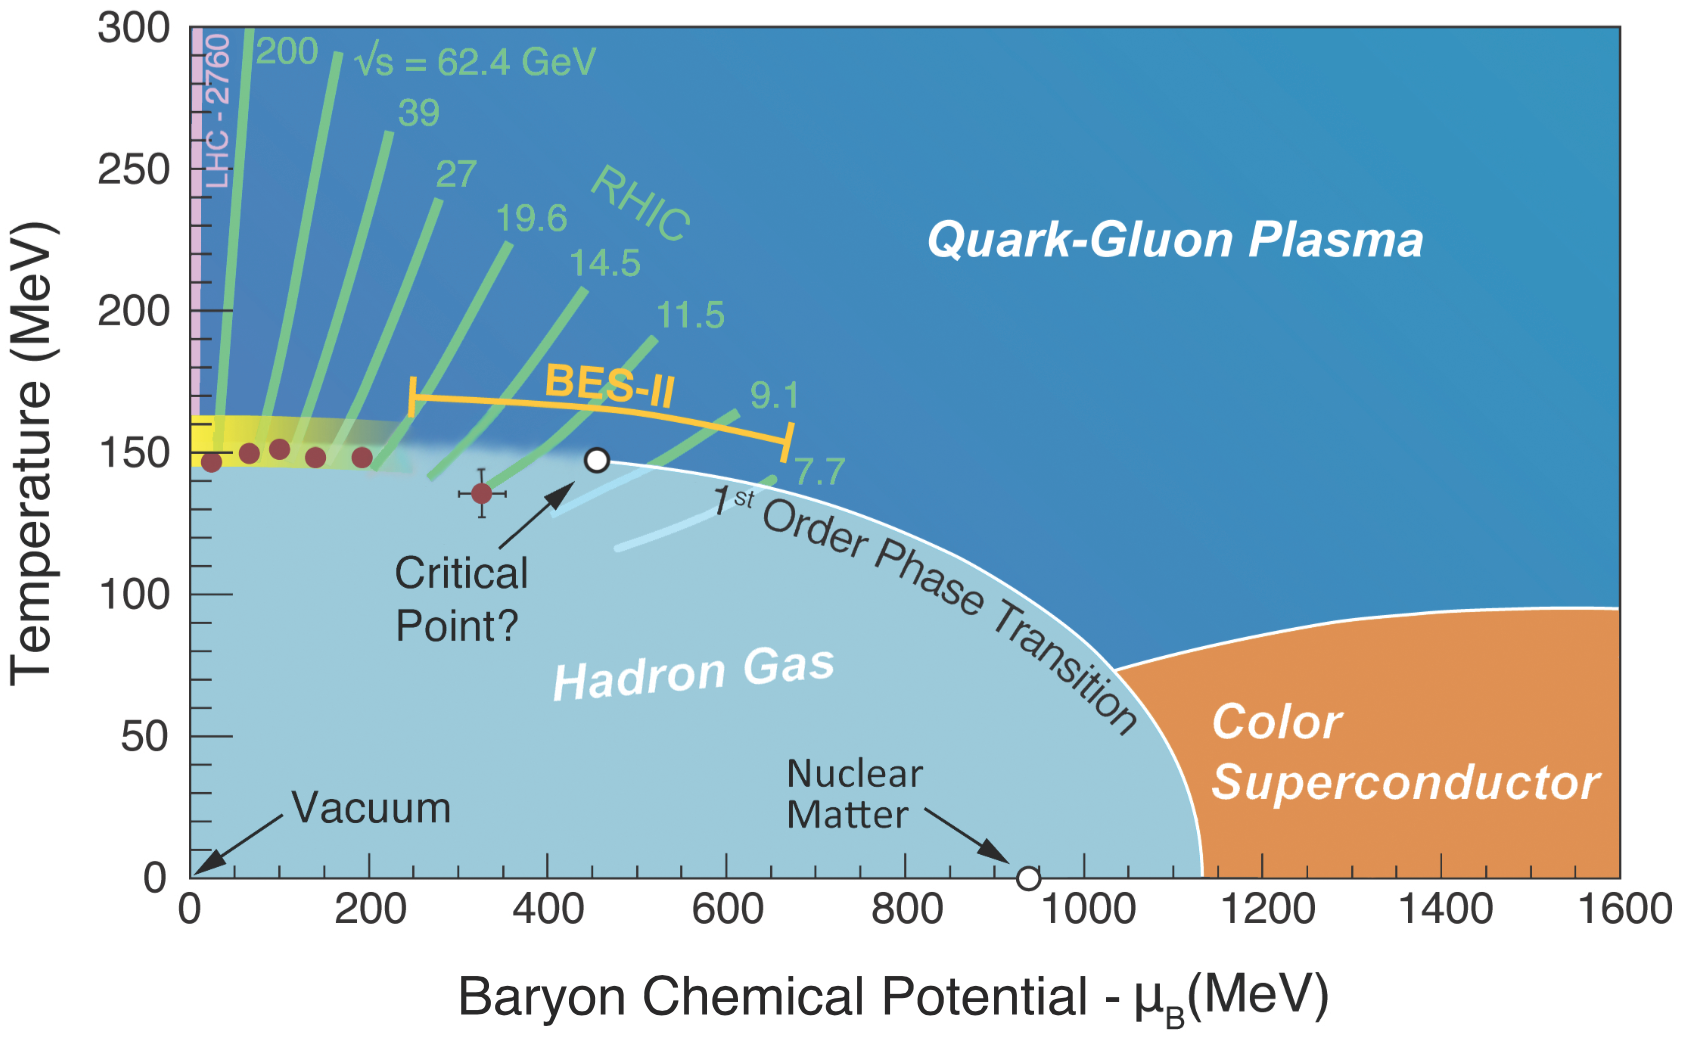
\includegraphics[width=.8\textwidth]{phase-diagram.png}
    \caption{Caption}
    \label{fig:phase-diagram}
\end{figure}
